\section{Datenbank (AW)}
\label{section_datenbank}
Als Datenbank kommt eine Instanz von MongoDB zum Einsatz.
Die Datenbank ist für Anwendung über die URI "mongodb://localhost:27017/img-server"{}zu erreichen.

Die Kommunikation zwischen Datenserver und Datenbank ist in Abbildung 
\ref{fig_kommunikation_datenbank} dargestellt.
\begin{figure}[h]
	\centering
	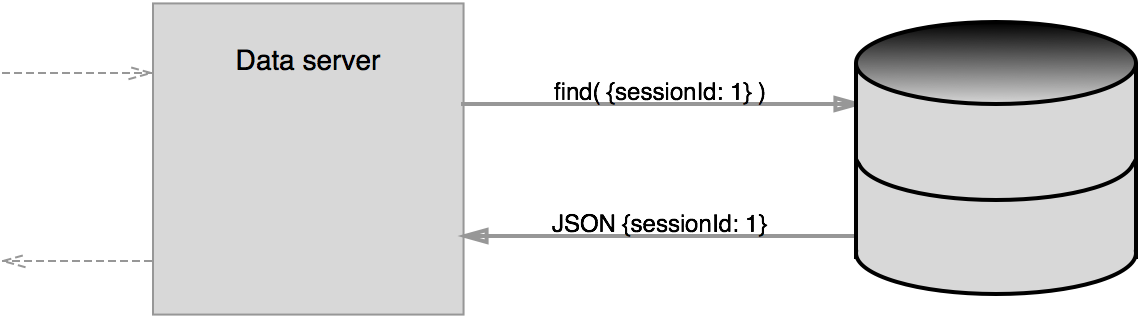
\includegraphics[width=14cm]{bilder/abbildung_datenbank}
	\caption{Kommunikation zwischen Datenserver und Datenbank}
	\label{fig_kommunikation_datenbank}
\end{figure}

Der Datenserver richtet Anfragen unter Verwendung des Moduls \textit{mongo-crud-layer}
an die Instanz von MongoDB. Da die Verkehrssprache von MongoDB JavaScript ist, können 
Anfragen aus der Datenserver-Anwendung heraus ohne eine weitere erstellt werden.

Das Modul \textit{mongo-crud-layer} stellt eine Abstraktion von CRUD-Operationen\footnote{Create, Read, Update, Delete} zur Verfü-gung.